\documentclass[12pt]{article}

\usepackage{preamble}



%title, author, date
\title{Netzwerkanalyse mit Wireshark: Welche (Meta-)daten werden weitergegeben?}
\author{Luis Herzog}
\date{April 2023}




\begin{document}





%Titlepage

\maketitle


\thispagestyle{empty}

\begin{figure}[h]
	\centering
	
\includegraphics[scale=0.1]{Bilder/Wireshark_icon.svg.png}
	\caption{Wireshark Logo}
	\label{fig:figure1}
\end{figure}


\newpage
\tableofcontents
\newpage

Es gibt viele verschiedenen Arten von Daten. Somit ebenfalls verschiedene Definitionen. 

Bevor man über die Wireshark Software sprechen kann, müssen die Basics geklärt werden:

\begin{itemize}
	\item Was sind Protokolle?
	\item Welche Protokolle gibt es?
	\item Wie funktionieren die Protokolle?
	\item das OSI Modell (IP/TCP)
	\item welcche Protokolle (welche können ausgelesen werden?
\end{itemize}
\section{Metadaten}
Metadaten sind tolle Daten \textbf{TODOO}
\subsection{Verwendungszwecke}



\section{Das Programm: Wireshark}
\subsection{Programm}


Wireshark ist eine Netzwerkpaketanalyse Software. Diese kann den aufgenommenen Netzwerktraffic in hohem Detail darstellen, um die Analyse dessen zu erleichtern. Die Darstellung der Ergebnisse erfolgt zum einen in Textform und zum anderen in Form von Grafiken, wie Diagrammen. Das Programm ist Open Source\footnote{Der Code des Programms ist öffentlich} und auf vielen Plattformen installierbar. Dazu gehören Windows, MacOS, Linux, Unix und BSD-Derivative. Im unteren Screenshot wird der Netzwerktraffic in einer VPN, in diesem Fall Mullvad VPN\footnote{\href{https://www.mullvad.net}{www.mullvad.net}} untersucht. Was direkt auffällt ist die Menge an Requests, die in nur wenigen Sekunden gesendet werden.

\begin{figure}[h]
	\begin{center}
		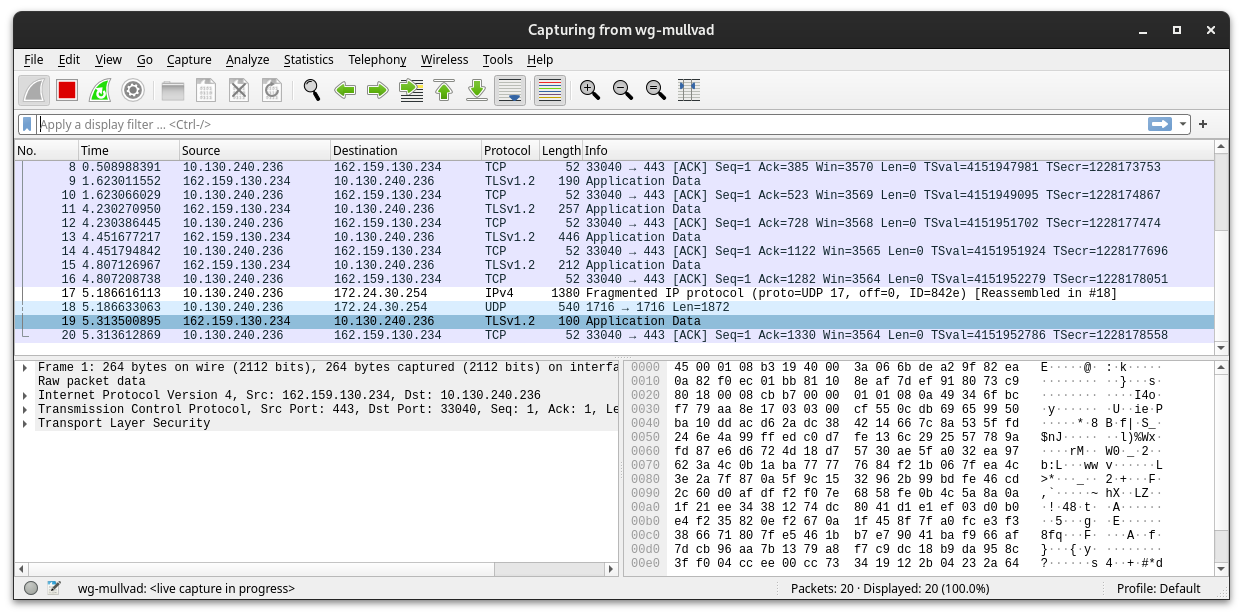
\includegraphics[scale=0.25]{Bilder/Screenshot_1.png}
		\label{fig:figure2}
		\caption{Beispielscreenshot aus der Wireshark Software}
	\end{center}
\end{figure}


\subsection{Funktionsumfang}

Wireshark ist eine Software mit sehr vielen Funktionen. Sie bietet wirklich alles rund um das Thema Netzwerkanalyse. Die wichtigsten Funktionen sind:
\begin{itemize}
	\item Die Verfügbarkeit aus sehr vielen Platformen
	\item Die Möglichkeit dumps von anderen Personen importieren zu können
	\item Das Filtern von Paketen nach sehr vielen Kriterien
\end{itemize}
Besonders die letztere Funktion ist sehr wichtig, da man ohne diese schnell die Orientierung in der Software verlieren kann. \cite{features}

\subsection{Anwendungsbereiche}
Wie im oberen Teil schon dargestellt, hat Wireshark sehr viele Funktionen. Allein deswegen wird es auch als Schweizer Taschenmesser der Netzwerktechnik bezeichnet. Somit kann Wireshark in sehr vielen Situationen Anwendung finden. Es kann beispielsweise von Netzwerk Administratoren benutzt werden, um Netzwerk Probleme  zu Analysieren und zu lösen. Es kann außerdem von Netzwerk Sicherheits Analysten benuzt werden, um Sicherheitsprobleme in Netzwerken zu finden. Wiederum kann es auch von Anwendungsentwicklern benutzt werden, um Netzwerkprotokoll Implementationen zu debuggen. Zuletzt kann es auch benutzt werden um mehr über Netzwerktraffic zu lernen und diesen zu Analysieren. Es gibt natürlich auch viele weitere Möglichkeiten WIreshark zu benutzen. \cite{intendedpurposes}




\newpage



\section{Netzwerk}

\subsection{Aufbau}
\subsection{Protokolle}
% tcp, udp, http(s), tls/ssl,  
% tor

\subsection{OSI Modell}


	% Please add the following required packages to your document preamble:
	% \usepackage{multirow}
\begin{wrapfigure}{r}{0pt}
	\centering
	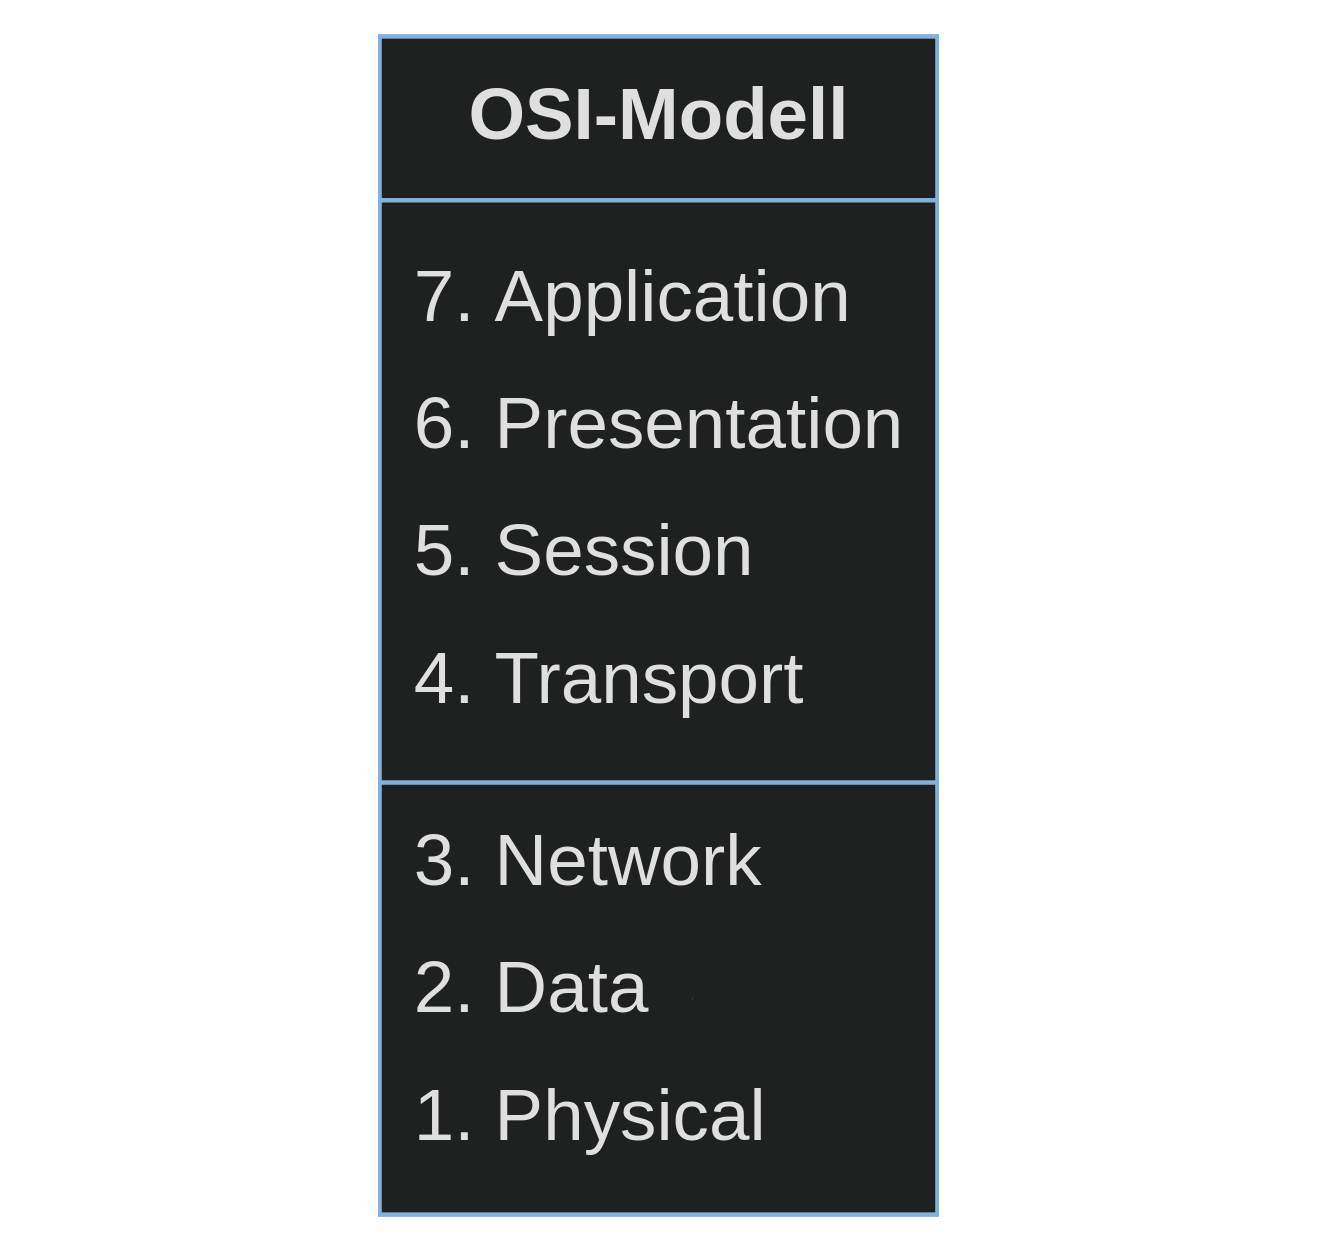
\includegraphics[scale=0.1]{Bilder/OSI-Modell}
	\caption{OSI-Modell}
	\label{fig:figure3}
	
\end{wrapfigure}



Das OSI-Modell wird benutzt, um den Aufbau eines Netzwerks zu vereinfachen, es ist ein tolles Werkzeug um das erstellen von sachen zu erleichtern



	
\subsubsection{Bitübertragungsschicht}
\subsubsection{Sicherungsschicht}
\subsubsection{Netzwerkschicht}
 \subsubsection{Transportschicht}
 \subsubsection{Sitzungsschicht}
 \subsubsection{Präsentationsschicht}
 \subsubsection{Anwendungsschicht}

\section{Analyse}
\subsection{Beispiel}
\subsection{Browser}
\subsubsection{Mozilla Firefox}
\subsubsection{Microsoft Edge}
 \subsubsection{Mullvad Browser}
\subsubsection{Opera Browser}




 \section{Fazit}

% end of text

\newpage
 \listoffigures
\newpage
\bibliographystyle{plain}
\bibliography{gg}

\newpage

\centering
\vspace*{200pt}
\Huge{\section{Anlagen}}

\end{document}

